\begin{SCfigure}[3][b]
  \centering
  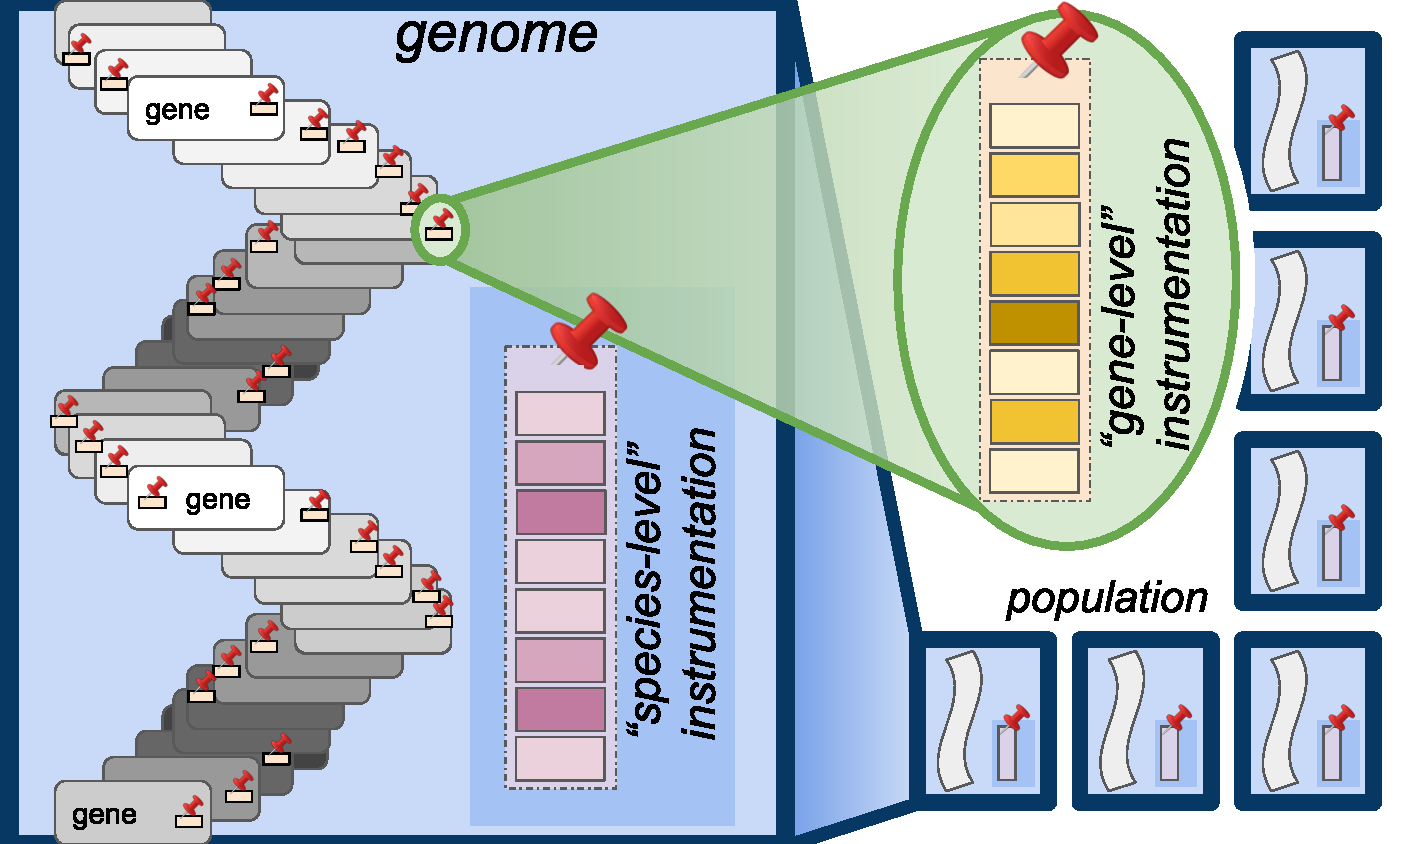
\includegraphics[width=0.5\textwidth]{img/annotation-types}
  \caption{
    Proposed instrumentation methods: ``species-level'' and ``gene-level'' instrumentation.
    Each organism has a single hereditary stratigraph attached as species-level instrumentation, with a gene drive mechanism (Figure \ref{fig:gene-drive}) ensuring consistentcy within species (i.e., interbreeding populations).
    Gene-level instrumentation associates instrumentation with individual genes, to be used for gene tree reconstructions.
  }
  \label{fig:annotation-types}
\end{SCfigure}
